\section{Restriction of Transformation Networks}

\mnote{Restrictions either transformation-local or for complete network}
We have discussed that it is necessary to restrict the transformations as an input of the application function to avoid that it is undecidable whether a consistent orchestration of them exists for given models and changes.
Those restrictions can be at two levels:
\begin{properdescription}
    \item[Transformation:] Restrictions only concern the single transformation. Thus, if each transformation fulfills a specific property, the application function is able to decide whether a consistent orchestration exists.
    \item[Network:] Restrictions concern the complete network, i.e., the combination of transformations. Only a set of transformations can have an appropriate property that enables the application function to decide the orchestration problem, but not each transformation on its own.
\end{properdescription}

\mnote{Find that all restrictions are impractical}
Since we assume transformations to be developed and reused independently, restrictions to single transformations are of special interest.
It is, however, easy to see that it will unlikely be possible to define practical restrictions to single transformations that make the orchestration problem decidable.
We will see that even impractical restrictions do not make the problem decidable.
Additionally, we discuss possible restrictions to complete networks.
We discuss properties that obviously provide the ability to avoid divergence and alternation in the states of a network, namely monotony and confluence.
Unfortunately, we will show that those restrictions are impractical.

% \todo{Maybe conflucence and monotony are rather restrictions of the application function (i.e. conservative operations) rather then restrictions of the transformation?}

% \begin{itemize}
%     \item Restrictions must, in the best case, be local to a transformation, i.e., they should be fulfillable without knowing with which other transformations the transformation shall be combined
%     \item Can this ever be the case?
% \end{itemize}

% \begin{itemize}
%     \item Discuss different restrictions we may apply to synchronizing transformations and networks
%     \item We conclude that none of them is practically
%     \item This does not mean that there is no restriction, but we were not able to find one
%     \item Maybe also discuss history-ignorance
% \end{itemize}

% Lösungsoptionen (Grad der Einschränkung an die Transformationen) --  überdeckt sich mit der Klassifizierung hierüber -> zusammenführen
% \begin{itemize}
%     \item Hohe Einschränkung: Jede beliebige Reihenfolge von ausgeführten Transformationen führt letztendlich zu einem korrekten Ergebnis (Fixpunktiteration -- Allquantifizierung) -- Hippokratie-Eigenschaft sorgt dafür, dass keine Transformation wieder etwas ändert, wenn Konsistenz bereits hergestellt ist.
%     Diese Eigenschaft ist in der Praxis möglicherweise zu strikt, da sie sehr starke Anforderungen an die Transformationen stellen müsste. Dafür wäre aber die Anwendungsfunktion trivial.
%     \item Mittlere Einschränkung: Es gibt eine Reihenfolge von ausgeführten Transformationen für jede Änderung die terminiert (Existenzquantifizierung) und die Ausführungsfunktion findet diese Reihenfolge.
%     Utopisch, dass die Anwendungsfunktion aus (potentiell sehr mächtigen) Transformationen die richtige Reihenfolge errechnen kann. Dafür aber (möglicherweise) weniger Anforderungen an die Transformationen (zumindest nicht mehr Anforderungen, denn die Allquantifizierung induziert die Existenzquantifizierung). Eine Funktion könnte dann zumindest nach best-effort versuchen, die richtige Reihenfolge zu finden und konservativ abbrechen, wenn sie diese nicht finden kann (also entweder konsistent terminieren oder terminieren mit der Aussage, dass es entweder keine solche Reihenfolge gibt -- bei relaxierten Anforderungen -- oder dass es sie nicht finden kann).  
%     \item Geringe Einschränkung: Es gibt potentiell keine Reihenfolge der Transformationen, die bei einer Änderung zu einer konsistenten Lösung kommt. Hier müsste die Ausführungsfunktion entsprechend einen Fehler ausgeben.
% \end{itemize}


\subsection{Options in Consistency Relations}

\mnote{Consistency preservation rules may select contradictory options in consistency relations}
We have seen in the examples and the discussion in \autoref{chap:orchestration:design_space:problem} that an essential reason for the non-existence of a consistent orchestration is the existence of options within consistency relations.
This means that a condition element is allowed to correspond to to different condition elements to be considered consistent, like we have seen for the mapping of names in \autoref{fig:orchestration:no_orchestration}.
Different transformations can define different such options for specific elements, such that some of these options can never exist in globally consistent models, but only the ones that overlap between the consistency relations of all transformations can occur there.
Compatibility of the consistency relations ensures that there is at least one such element in the overlap of the consistency relations, because if there was no consistent set of models containing the condition element the relations would be considered incompatible.
Unfortunately, each transformation can only select one of these options to restore consistency when a condition element is added and if all transformations choose an element that is not in the overlap of the consistency relations, they will never find a consistent set of models.

\mnote{Reduce expressiveness by each condition element only in one consistency relation pair}
In consequence, an obvious option to reduce expressiveness of transformations in order to make the orchestration problem decidable by ensuring that a consistent orchestration does always exist would be to restrict consistency relations, such that each condition element is only allowed to occur in a single consistency relation pair of a consistency relation.
Thus, each condition element has a unique corresponding element to which it is considered consistent.
Then, the consistency preservation rules cannot select between different options to restore consistency and if the relations are compatible, all consistency relations relate elements in an equal way, thus the transformations must find exactly those elements.

\mnote{Consistency relation restriction does not solve the problem}
Although that approach will at least reduce the number of cases in which no consistent orchestration is found in our algorithm, there are still inputs for which no consistent orchestration exists.
Since we do not restrict the transformation in what they are allowed to do, they can perform arbitrary changes to restore consistency.
This especially includes that they may always returns changes that yield the same two models, which are consistent to that transformation but not to any models that can be delivered by the other transformations.
% Since we do not restrict the transformation in what they are allowed to do, they can perform arbitrary changes that restore consistency, such that alternations in the execution can occur.
% Consider three metamodels $\metamodel{A}, \metamodel{B}, \metamodel{C}$ with the following consistency relations and consistency preservation rules:
% \begin{align*}
%     &
%     \consistencyrelation{CR}{AB} = \setted{\tupled{\model{a}{1}, \model{b}{1}}, \tupled{\model{a}{2}, \model{b}{3}}, \tupled{\model{a}{3}, \model{b}{2}, \tupled{\model{a}{4}, \model{b}{4}} \\
%     &
%     \consistencypreservationrule{\consistencyrelation{AB}}(\model{a}, \model{b}, \change{\metamodel{A}}, \change{\metamodel{B}}) = \begin{cases}
%     \end{cases}
%     &
%     \consistencyrelation{CR}{BC} = \setted{\tupled{\model{b}{1}, \model{c}{1}}, \tupled{\model{b}{2}, \model{c}{3}}, \tupled{\model{b}{3}, \model{c}{2}, \tupled{\model{b}{4}, \model{c}{4}} \\
%     &
%     \consistencyrelation{CR}{AC} = \setted{\tupled{\model{a}{1}, \model{c}{1}}, \tupled{\model{a}{2}, \model{c}{3}}, \tupled{\model{a}{3}, \model{c}{2}, \tupled{\model{a}{4}, \model{c}{4}} \\
% \end{align*}

\mnote{Example with restriction but without consistent orchestration}
Let $\class{A}{}$, $\class{B}{}$, $\class{C}{}$ be three classes, each with one attribute $n$ storing a number.
We define the following metamodels, each only consisting of one of those classes, and consistency relations between them that define that for each element in one model a corresponding the others with the same value of $n$ has to exist.
These consistency relations are obviously compatible.
This is a further simplification of our running example that requires persons, residents and employees with the same names.
Additionally, we define consistency preservation rules, each of them delivering changes that always, i.e., for every input, yield the same models that only consist of one element with a specific value.
The resulting models are chosen in a way such that they are consistent to the according consistency relation, but not to any of the others.
\begin{align*}
    & 
    \metamodelinstanceset{M}{1} = \mathcal{P}(\metamodelinstances{\class{A}{}}), %\\
    %& 
    \metamodelinstanceset{M}{2} = \mathcal{P}(\metamodelinstances{\class{B}{}}), %\\
    %& 
    \metamodelinstanceset{M}{3} = \mathcal{P}(\metamodelinstances{\class{C}{}}) \\[1em]
    &
    \consistencyrelation{CR}{12} = \setted{\tupled{a,b} \in \metamodelinstances{\class{A}{}} \times \metamodelinstances{\class{B}{}} \mid a.n = b.n}, \consistencyrelationset{CR}_{12} = \setted{\consistencyrelation{CR}{12}, \consistencyrelation{CR}{12}^T} \\
    &
    \consistencypreservationrule{\consistencyrelationset{CR}_{12}}(\model{m}{1}, \model{m}{2}, \change{\metamodel{M}{1}}, \change{\metamodel{M}{2}}) = (\change{\metamodel{M}{1}}', \change{\metamodel{M}{2}}') \\
    & \formulaskip
        \mathtext{with} \change{\metamodel{M}{1}}'(\model{m}{1}) = \setted{a \in \metamodelinstances{\class{A}{}} \mid a.n = 1} \land \change{\metamodel{M}{2}}'(\model{m}{2}) = \setted{b \in \metamodelinstances{\class{B}{}} \mid b.n = 1} \\[1em]
    &
    \consistencyrelation{CR}{13} = \setted{\tupled{a,c} \in \metamodelinstances{\class{A}{}} \times \metamodelinstances{\class{C}{}} \mid a.n = c.n}, \consistencyrelationset{CR}_{13} = \setted{\consistencyrelation{CR}{13}, \consistencyrelation{CR}{13}^T} \\
    &
    \consistencypreservationrule{\consistencyrelationset{CR}_{13}}(\model{m}{1}, \model{m}{2}, \change{\metamodel{M}{1}}, \change{\metamodel{M}{3}}) = (\change{\metamodel{M}{1}}', \change{\metamodel{M}{3}}') \\
    & \formulaskip
        \mathtext{with} \change{\metamodel{M}{1}}'(\model{m}{1}) = \setted{a \in \metamodelinstances{\class{A}{}} \mid a.n = 2} \land \change{\metamodel{M}{3}}'(\model{m}{3}) = \setted{b \in \metamodelinstances{\class{C}{}} \mid c.n = 2} \\[1em]
    &
    \consistencyrelation{CR}{23} = \setted{\tupled{b,c} \in \metamodelinstances{\class{B}{}} \times \metamodelinstances{\class{C}{}} \mid b.n = c.n}, \consistencyrelationset{CR}_{23} = \setted{\consistencyrelation{CR}{23}, \consistencyrelation{CR}{23}^T} \\
    &
    \consistencypreservationrule{\consistencyrelationset{CR}_{23}}(\model{m}{2}, \model{m}{3}, \change{\metamodel{M}{2}}, \change{\metamodel{M}{3}}) = (\change{\metamodel{M}{2}}', \change{\metamodel{M}{3}}') \\
    & \formulaskip
        \mathtext{with} \change{\metamodel{M}{2}}'(\model{m}{3}) = \setted{b \in \metamodelinstances{\class{B}{}} \mid b.n = 3} \land \change{\metamodel{M}{3}}'(\model{m}{3}) = \setted{c \in \metamodelinstances{\class{C}{}} \mid c.n = 3}
\end{align*}

\mnote{Consistency preservation rules always yield models not consistent to other relations}
The given consistency relations are compatible, they contain each condition element only in one consistency relation pair, and the consistency preservation rules are correct, as their result is consistent to the consistency relation.
Still, there is no consistent orchestration of the transformation for any input that is not yet consistent.
This is because the consistency preservation rules always produce models that are not consistent to the consistency relations between the other models.

\mnote{Exemplary consistency preservation rules perform unreasonable changes}
One might argue that the defined consistency preservation rules are highly unreasonable and will never occur in that way in practice.
We would probably assume the consistency preservation rules to preserve the input models and changes in some way instead of returning models that are completely unrelated with the input.
However, we not yet have an appropriate notion for that.
Some were on transformations, such as \cite{cheney2017LeastChangeBx-JOT,macedo2016alloy}, proposes a notion of \emph{least change} to ensure that transformations do not perform arbitrary unrelated changes, which could exclude that situations.

\mnote{Restriction of consistency relations is impractical}
Although the given example is rather artificial and although there might be the additional property of least change, which could further reduce the cases in which no consistent orchestration exists, the essential drawback is that these restrictions are not reasonable.
Allowing a condition element to occur in multiple consistency relation pairs is essential, because options for elements to considered is necessary, especially if there is a gap in the abstraction of two related metamodels.
For example, a UML class needs to be able to correspond to all Java classes that provide different implementations of that class.
Requiring that there is exactly one Java class that is considered consistent to a UML class is obviously not applicable in practice, thus this restriction would make the consistency notion useless.

\mnote{Least change property does even not solve the problem}
If we, instead, only require some notion of least change, such as that only elements are changed which are involved in a violated consistency relation, this does also not solve the problem.
In the example in \autoref{fig:orchestration:no_orchestration}, relating the names of employees, residents and persons, we have defined consistency preservation rules that only require changes to elements that actually violate consistency.
Nevertheless, we have shown that for these consistency preservation rules only specific orchestrations are consistent and that with some modification even no consistent orchestration exists.

\mnote{Unlikely to find practical restrictions that solve the problem}
In consequence, we found that even a well-defined restriction that is too strong to be applied in practice still cannot ensure that a consistent orchestration exists for possible every input, even if the examples with used to show that on are rather artificial.
Although this does not serve as a proof for the impossibility for find a suitable restriction that solves the orchestration problem, which is even impossible because there is no unique notion of what an acceptable restriction would be, the investigated case shows that it is unlikely to find practical restrictions that solve the problem, if even impractical restrictions do not solve it.

% Es kann z.B. sein, dass ein Element a ein Element b braucht. Eine andere Transformation braucht zwei as und dafür ein (oder zwei) c. Dann ist (a,b) konsistent und es ist auch kompatibel, weil es mit dem a ein Modell gibt in dem es konsistent ist, nämlich das mit dem zweiten a, aber das Modell mit einem a ist nur lokal konsistent. Wenn das nun immer von der Transformation ausgewählt wird, findet man nie einen konsistenten Zustand.

% - We have seen that selection of options is a problem that leads to the non-existence of orchestrations.
% - Intended solution: Each object may only have one corresponding element. Then if the object exists, exactly one other has to exist. This ensure that for any model a there is only exactly one consistent b.
% It can, however, be that a1, b1 and c1 are consistent and a4, b4 and c4 are, but only (a2, b3), (a3, b2), (a2, c3), (a3, c2), (b2, c3), (c3, b2) are consistent. 
% The relations may still be compatible, because for example (a2, b3, a4), (a3, b2, a5) and so ond could be consistent.
% Since we have no requirements such as a least change requirement, the transformation may, for every input, return one of the last pairs, although this actually does not make any sense.
% Then the transformations do only alternate between those models.
% This seems to be a rather theoretical consideration, because transformations will usually not perform arbitrary unreasonable changes, such as always returning the same models.
% However, even if we found that we can define an additional property, such as least change, such that requiring each object to only have one corresponding element in the consistency relations together with that property, then still the latter requirement is impractical, as usually an element can correspond to different others.
% At least in the case when consistency relations gap abstraction levels, this is necessary.
% For example, a UML class needs to be able to correspond to a Java class with any implementation of its bodies. Restricting it to only one is not practical.

% Although the restriction of relations is already an impractical restriction, it does still not solve the problem.
% Thus it is unlikely to find restrictions that are practical and solve the problem, although, for sure, it is not formally proven.

% Even some notion of least change that ensure that only elements are changed which are involved in any violated consistency relations will not be sufficient, as the example in \autoref{fig:orchestration:no_orchestration} has shown.
% There, only elements that are involved in the violated consistency relations are changed.
%One might argue that in that example the consistency relations contain pairs of elements that can never be created by the consistency preservation rules and thus should not be part of the consistency relations.
%Gegenargument: Es gibt oft unendlich viele Paare (z.B. alle Implementierung einer Java Klasse mit einer UML-Klasse. Wenn auf der UML-Seite auch noch ein Freiheitsgrad ist, dann wird jede UML-Instanz der Klasse auf eine Standard Java-Klasse abgebildet und jede Java-Klasse auf eine Standard UML-Klasse, aber die Zusatzinformationen kommen erst durch manuellen Anreicherung dazu und sind dadurch vorhanden, aber nicht durch die Transformation)


\subsection{Confluence}
%\todo{Zeigen: Konfluenz führt zu Konvergenz. Aber konfluenz ist zu starke Anforderung, außerdem heißt Konvergenz, dass egal welche Reihenfolge der Transformationen man wählt am Ende immer das gleiche Ergebnis rauskommt. Das muss aber nicht so sein. Gebe Beispiel mit groß klein Schreibung, wo je nach Reihe folge verschieden elosungen rauskommen}
%\todo{Diss: Konvergenz einführen, hinreichende Eigenschaft? Notwendige Eigenschaft?}
%\todo{Discuss confluence and convergence!}

\begin{figure}
    \centering
    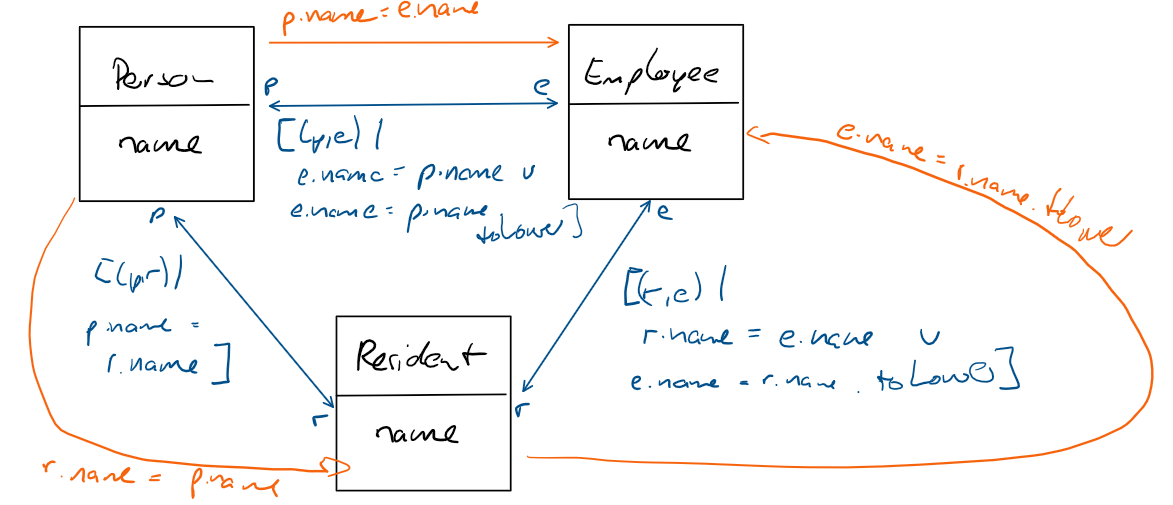
\includegraphics[width=\textwidth]{figures/correctness/orchestration/confluence.png}
    \caption[Confluence of transformations]{Counterexample for the practicality of confluence}.
    \label{fig:orchestration:confluence}
\end{figure}

In literature~\cite{stevens2020BidirectionalTransformationLarge-SoSym}, confluence in a transformation network is described as the property that two consistent orchestrations for the same given models and changes always yield the same models.
Thus, executing transformations in any order such that the result is consistent will deliver the same result.
It is, however, easy to see that this is an impractical requirement.

In the example depicted in \autoref{fig:orchestration:confluence}, derived from the running example, three consistency relations expect for each person, employee and resident two corresponding others to exist.
They need to have the same name or, in case of the relations between persons and employees, as well as between residents and employees, the employee may have the same name in lower case.
The consistency preservation rule between persons and employees ensures that an employee with the same name exists, whereas the one between residents and employees ensures that an employee with the name in lower case exists.
Whenever a person is added, two consistent orchestrations can be distinguished.
First, the transformation between persons and employees can be executed, either followed or preceded by the one between persons and residents. Then all elements have the same name.
The models are also consistent to the relation between residents and employees, because the relation allows the names to be equal.
Second, the transformation between persons and residents can be executed, followed by the one between residents and employees.
Then the employee has the name in lower case, but still this is consistent to the relation between persons and employees.

Apart from that artificial example, such a situation can always occur if transformations have different options for elements to be consistent.
If there is not a single element that is in the overlap of consistent elements between all transformations, the result may be any of the elements in the overlap.
And the result may depend on which transformation made the first selection that fell into the overlap.
Finally, \textcite[p. 14]{stevens2020BidirectionalTransformationLarge-SoSym} also states explicitly that a network will only be confluent under very specific circumstances.

% Another intuitive notion of confluence would require that information flows together in a compatible way, i.e., the execution of a transformation does not violate consistency to other adjacent transformations.
% Formally this can be described as: A network is confluent when in every cycle of transformations t1,...tn the execution t1...ti-1 and tn,...,ti for any i leads to the same changes in the network.
% This means it does not matter in which order two transformations propagating information to the same model are executed.
% This, in consequence, means that the execution of a transformation cycles always yields models that are consistent to all transformations. Although two transformations affected the same model, consistency to the earlier executed one is not destroyed again.
% Finally, this reduces to the situation that executing each transformation once restores consistency to all transformations, which is, as we have seen, impractical.



\subsection{Monotony}

\begin{itemize}
    \item Muss eine Transformation mit jedem beliebigen Delta umgehen können müssen? Eine Einschränkung auf Monotonie würde dies verhindern. Bzw. wir müssten zeigen, dass es Konsistenzrelationen gibt, die unter der Anforderung an Monotonie nicht wiederhergestellt werden können. Bspw. fügt eine andere Transformation 3 Elemente hinzu, wo zwei mit dem anderen entsprechend der Konsistenzrelationen korrelieren und somit keine Witness-Struktur aufgebaut werden kann, die Konsistenz beweist. Das lässt sich durch Hinzufügen weiterer Elemente potentiell nicht auflösen (siehe Beispiele im SoSym-Paper).
    \item Refer to synchronization chapter, where we introduced a monotony notion based on transformations being partial-consistency-improving. Here, in contrast, the CPRs cannot be aligned, such that we cannot, for example, expect one transformation not to lead to a reduction of consistency regarding consistency relations of other, previously executed transformations.
\end{itemize}
\begin{itemize}
    \item Im Allgemeinen könnte eine Transformation beliebige dieser Deltasequenzen modifizieren. Wir verlangen jedoch, dass eine Transformation nur Deltas anhängt, also die Sequenzen länger werden
    \item Genauer beschränken wir auch, welche Sequenzen eine Transformation sehen und ändern darf, genau gesagt darf sie die Sequenzen von zwei Modellen sehen und eine davon verlängern.
    \item Hier kommt bereits der Unterschied zu bisherigen Transformationen, denn die sehen nur Deltas an einem Modell und erzeugen Deltas an dem anderen. Das ist bei uns schon gänzlich anders. Bidirektionale Transformationen unterstützen das im Übrigen auch nicht, sondern sind nur Spezifikationen, aus denen sich Wiederherstellungsroutinen für beide Richtungen ableiten lassen (siehe Stevens 2010)
\end{itemize}

\paragraph{Idea:} Require monotony to avoid alternation

We would have to relax the definition of transformation to be monotone, because if a transformation is monotone, it may only append information, but this is not always possible, as can be seen in the following example. A monotone transformation must be able to return bottom if it cannot make further changes to restore consistency to the relation.

\begin{definition}[Monotone Transformation]
    Transformation gets models M and deltas D and produces new deltas D'. Taking the union of the original models M and the new models D'(M), then D(M) must be a subset of that, because other elements would have been added and removed afterwards or elements would have been changes once by D and again in a different way by D'.

    Generally, monotony could also mean that only the same complete model state is not passed twice. \todo{Why dont we do that?}
\end{definition}

This would mean that each transformation only appends changes, i.e., if an element was added/removed, the transformation may not do the inverse. The same applies to attribute/reference changes: if an attribute/reference was already changes it may not be changed again.
This way, it is by design impossible to pass through the same state again. Actually, if a monotone transformation returns bottom, the network has to terminate with a failure.
However, this is hard restriction to transformations. It leads to the fact that in some networks that actually have a simple solution no solution is found at all. This can be easily seen at the example in \autoref{fig:formal:monotonycounterexample}. In the example adding "aa" to the left model, any execution order of the transformations leads to the situation that a previous change must be revoked to result in a consistent state. However, it is possible to derive a consistent state for that input change.

\begin{figure}
    \centering
    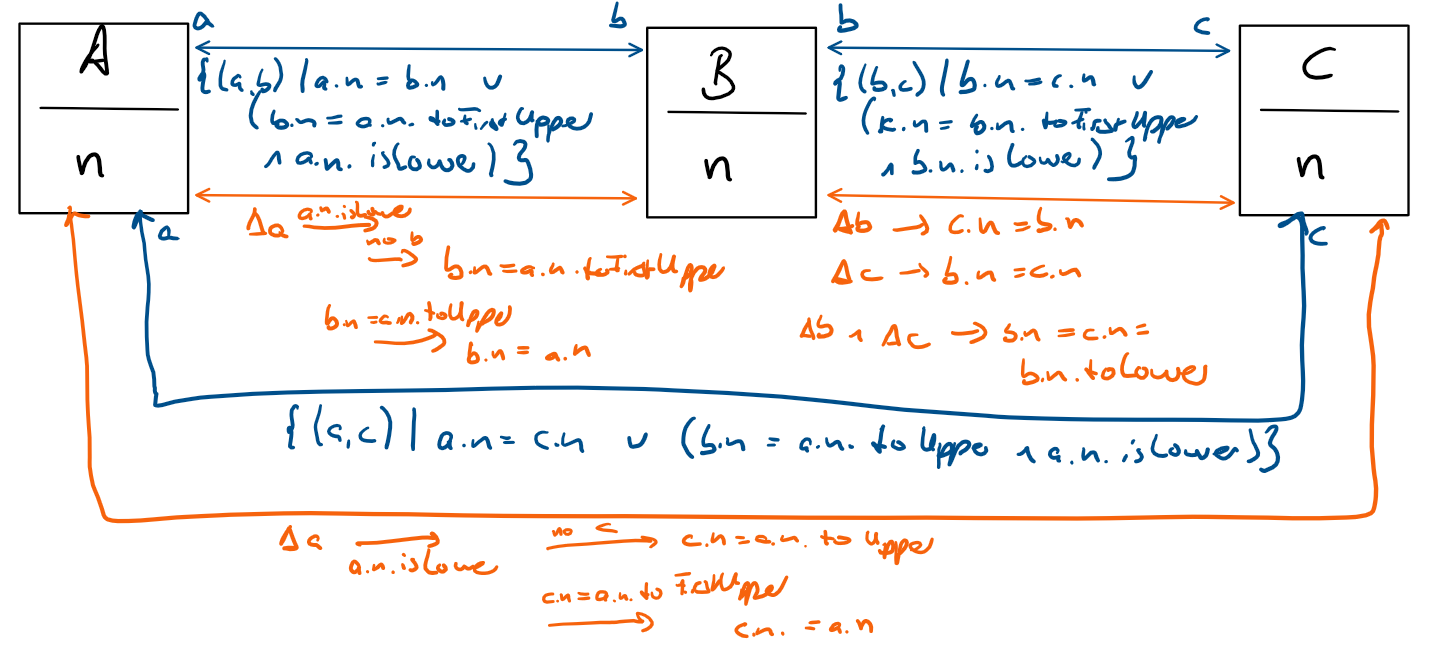
\includegraphics[width=\textwidth]{figures/correctness/orchestration/monotony_counterexample.png}
    \caption{Counterexample for monotony}
    \label{fig:formal:monotonycounterexample}
\end{figure}

One could now argue that there are binary relations in the example, which may never be fulfilled at all. We will later discuss how far relations that cannot be fulfilled should be restricted. However, in general, this is wanted behavior, because in general it may be necessary that transformations produce intermediate states that are not yet consistent with each other. Otherwise this would means that each transformation is always able to directly deliver a state that is consistent to all other relations, which is especially not possible, because other transformations may add further information to the models. More precisely, a relation may consider <a model consistent to all other models that contain any additional information not affected by the transformation. For example, a UML class model may be considered consistent to all Java models with any implementation of the specified methods, thus to an infinite number of models. Now saying that it should not be allowed that the transformation selects one with an empty implementation because that is not consistent to another relations induced by another transformation, such as the relationship to a component model, does not make any sense. Thus having those relation elements that may be considered locally consistent but will never occur in a globally consistent tuple of models does not make sense.
In the example, we can see that such an inconsistent intermediate state is passed through and afterwards a consistent tuple of models is reached if not requiring monotony.
In consequence, requiring monotony from transformations is a too strict requirement, because it is necessary to run through states that may be changed later on.

\begin{theorem}
    An application function for monotone transformations either returns a consistent model or produce a sequence of CPRs returning delta that return models of always growing size (i.e. it diverges).
\end{theorem}

\paragraph{Divergence cannot be avoided}

There are rather equal network, one that terminates after a long time and one that never terminates. 
Consider the example. The relations are defined in a way such that for any allocation for any of them a consistent tuple of models can be found. However, the transformations are not able to find it because they make "bad" choices from a set of choices that are conflicting. 
This can be seen in the example that we have already given in \autoref{fig:correctness:no_execution_order}.

Thus, systematically avoiding divergence is not possible. 

\textbf{Central insight:} Alternation / Divergence cannot be avoided systematically (like in ordinary programming), if not restricting transformations in a way that may not be reasonable.



% \subsection{Unresolvability}

% Discuss why no execution order may exist although relations are compatible.
% If not even an order exists, the application function or the algorithm can, for sure, not find it.

% However, we found that we cannot always find an execution order if it exists and we were not able to find restrictions to transformations to ensure that it exists.
% We expect the same for the existence of an execution order at all.
% All restrictions we can make are likely to be too restrictive.
% The problem arises when there is an overlap of consistent models between some transformations, but they always decide for other elements that are not in the overlap of consistent models.
% It would, obviously, require the transformation to know about the others to ensure that this is not the case.
% This conflicts our assumption.

% Finally, it may be valid that for some changes no execution exists, because the change can not be processed on purpose \todo{Give example for that!}.
% Should this be the case if we assume compatibility?

% Although a more detailed investigation of the claim that we cannot define reasonable requirements to the transformations to ensure that they can always be ordered to restore consistency is a topic for further research, we did not investigate it in the scope of this thesis.
% Since we found it necessary to find a conservative algorithm that can deal with the case that no execution is found anyway, that algorithm covers the case that no execution order exists as well and thus is a solution for this problem as well.

% Beispiel:
% \begin{itemize}
%     \item Das ist im allgemeinen aber nicht Fall. Letztendlich trifft jede Transformation lokale Entscheidungen. Beispielsweise könnte jede einzelne Transformation gegeben eine beliebige Änderung immer dieselben Modelle (bzw. Änderungen die dazu führen) zurück liefern (im trivialsten Fall leere Modelle). Dann erfüllt jede Transformation ihre Korrektheitseigenschaft bzgl. ihrer Relation, aber das Netzwerk muss nicht korrekt sein, da bspw. T(A,B) und T(B,C) sich immer für verschiedene Instanzen von B entscheiden. Es gäbe somit nie eine konsistente Lösung für eine beliebige Ausführungsreihenfolge der Transformationen, auch wenn die Relationen das erlauben würden.
%     \item Beispiel mit Namen, wo eine Transformation immer den großen Namen zurück liefert, die andere immer den kleinen. T(A,B) bildet A auf gleiches B ab und beide auf kleine Schreibweise, obwohl beide erlaubt sind. Erzeuge A="a", dadurch B="a". T(B,C) bildet B auf C ab und beide auf große Schreibweise, obwohl beide erlaubt sind. Somit macht sie das zu B="A" und C="A". Nun wird T(A,B) wieder beide klein machen usw. Allerdings wäre eine insgesamt valide Lösung einfach alle groß oder alle klein zu machen, aber die Transformationen finden diesen Zustand nicht. 
% \end{itemize}